\documentclass[a4paper, 12pt]{article}

\usepackage{custom}

%--------------------VARIABILI--------------------
\def\lastversion{v1.3}
\def\title{Analisi dei requisiti}
\def\date{21 Marzo 2025}
%------------------------------------------------

\begin{document}

\primapagina


\begin{registromodifiche}
    \lastversion & 21 Marzo 2024 & Marko Peric, Francesco Savio, Eghosa Matteo Igbinedion Osamwonyi, Enrico Bianchi, Guirong Lan & Pedro Leoni & Sezioni \hyperref[sec:use_case]{Use case}, \hyperref[subsec:requisiti_funzionali]{Requisiti funzionali}, \hyperref[subsec:requisiti_non_funzionali]{Requisiti non funzionali}\\
    \hline
    v1.2 & 12 Marzo 2024 & Marko Peric & Eghosa Matteo Igbinedion Osamwonyi & Sezione \hyperref[sec:introduzione]{Introduzione}\\
    \hline
    v1.1 & 10 Marzo 2025 & Pedro Leoni & Marko Peric & Sezioni \hyperref[sec:requisiti_utente]{Requisiti utente}, \hyperref[sec:requisiti_software]{Requisiti software}, \hyperref[subsec:requisiti_funzionali]{Requisiti funzionali}, \hyperref[subsec:requisiti_non_funzionali]{Requisiti non funzionali}\\
    \hline
    v1.0 & 3 Marzo 2024 & Marko Peric & Francesco Savio & Release\\
    \hline
    v0.4 & 28 Febbraio 2025  & Pedro Leoni, Enrico Bianchi & Francesco Savio, Marko Peric & Sezioni \hyperref[sec:use_case]{Use case}, \hyperref[sec:requisiti_software]{Requisiti software} \\
    \hline
    v0.3 & 12 Gennaio 2025 & Pedro Leoni, Francesco Savio, Guirong Lan & Marko Peric & Sezione \hyperref[sec:requisiti_software]{Requisiti Software} \\
    \hline
    v0.2 & 8 Gennaio 2025 & Pedro Leoni, Francesco Savio & Marko Peric & Sezioni \hyperref[sec:requisiti_utente]{Requisiti utente} \hyperref[sec:use_case]{Use case} \\
    \hline
    v0.1 & 13 Dicembre 2024  & Pedro Leoni & Enrico Bianchi & Sezioni \hyperref[sec:descrizione_prodotto]{Descrizione prodotto} \\
    \hline
\end{registromodifiche}

\tableofcontents

\newpage

\section{Introduzione}
\label{sec:introduzione}

\subsection{Scopo del documento}
\label{subsec:ScopoDelDocumento}
Il presente documento offre un'analisi approfondita dei casi d'uso e dei requisiti del progetto Artificial QI, in linea con gli standard e le convenzioni dell'ingegneria del software. 
L'analisi è stata sviluppata a partire dal capitolato C1 presentato dalla Proponente Zucchetti S.p.A., arricchita da una collaborazione attiva durante gli incontri dedicati. 
L'obiettivo principale è delineare le funzionalità e le caratteristiche dell'applicativo, fornendo una base solida per la successiva progettazione del sistema.

\subsection{Riferimenti}
\label{subsec:Riferimenti}

\subsubsection{Riferimenti normativi}
\label{subsubsec:RiferimentiNormativi}
\begin{itemize}
    \item Norme di Progetto v0.14;
    \item Corso di Ingegneria del Software - Regolamento del Progetto Didattico:
    \newline
    \href{https://www.math.unipd.it/~tullio/IS-1/2024/Dispense/PD1.pdf}{Slide del corso di Ingegneria del Software};
\end{itemize}

\subsubsection{Riferimenti informativi}
\label{subsubsec:RiferimentiInformativi}
\begin{itemize}
    \item Capitolato d'appalto C1 - Artificial QI:
    
    \href{https://www.math.unipd.it/~tullio/IS-1/2024/Progetto/C1.pdf}{Testo del capitolato C1}
    
    \href{https://www.math.unipd.it/~tullio/IS-1/2024/Progetto/C1p.pdf}{Presentazione del capitolato C1}
    
    \item Slide del corso di Ingegneria del Software: T5 - Analisi dei Requisiti:
    
    \href{https://www.math.unipd.it/~tullio/IS-1/2024/Dispense/T05.pdf}{Dispensa T05}
    
    \item Glossario v0.3
    
    \item Verbali interni:
    \begin{itemize}
        \item 2024/11/21;
        \item 2024/11/25;
        \item 2024/11/28;
        \item 2024/12/10;
        \item 2024/12/19;
        \item 2024/12/26;
        \item 2025/01/04;
        \item 2025/01/09;
        \item 2025/01/23;
        \item 2025/02/24.
    \end{itemize}
    
    \item Verbali esterni:
    \begin{itemize}
        \item 2024/12/05;
        \item 2025/01/13.
    \end{itemize}
\end{itemize}

\subsubsection{Riferimenti esterni}
\label{subsubsubsec:RiferimentiEsterni}
\begin{itemize}
    \item \textit{Learning UML 2.0}, di Russell Miles, O'Reilly Media, 2006;
    \item Approfondimento su diagrammi dei casi d'uso:
    
    \href{https://www.geeksforgeeks.org/use-case-diagram/}{geeksforgeeks.org};

\end{itemize}

\subsection{Glossario}
\label{subsec:glossario}
Per prevenire eventuali incomprensioni legate al linguaggio utilizzato nella documentazione di progetto, viene messo a disposizione un Glossario, in cui ogni termine è accompagnato da una spiegazione volta a chiarirne il significato. 
I termini tecnici, gli acronimi e le parole potenzialmente ambigue sono formattati in corsivo all'interno dei documenti e contrassegnati da una lettera \glossario{ } in pedice. 
Tale formattazione viene applicata a tutte le occorrenze dei termini definiti nel Glossario.

\section{Descrizione del prodotto}
\label{sec:descrizione_prodotto}


\subsection{Obiettivi del prodotto}
L'obiettivo del prodotto è permettere la valutazione automatica delle prestazioni di un \glossario{Large Language Model} su un \glossario{dataset} composto da un insieme di coppie domanda-risposta.
Il sistema permetterà la riduzione/eliminazione della verifica umana diminuendo i costi dei test delle prestazioni su questi modelli di linguaggio.
Il sistema prodotto può quindi essere usato per:
\begin{enumerate}
    \item Confrontare le prestazioni di diversi \glossario{Large Language Model}.
    \item Confrontare le implicazioni prestazionali di diverse scelte implementative di un \glossario{Large Language Model}.
\end{enumerate} 
Il prodotto verrà quindi utilizzato per prendere decisioni sull'integrazione e l'implementazione di \glossario{Large Language Model}.


\subsection{Funzioni del prodotto}
Le funzioni principali del sistema sono:
\begin{itemize}
    \item Gestione del dataset: inserimento, modifica ed eliminazione delle coppie di domanda e risposta su cui eseguire il test.
    \item Persistenza del dataset: caricare e memorizzare il dataset.
    \item Sottoporre le domande al modello da testare: interfacciarsi al modello esterno tramite un \glossario{API REST} documentata secondo lo standard \glossario{OpenAPI 3.1}.
    \item Eseguire il test: deve riuscire a valutare la correttezza/verosimiglianza delle risposte ricevute dal modello sottoposto al test in base alle risposte attese.
    \item Mostrare i risultati del test: i risultati devono essere mostrati usando una \glossario{dashboard} che mostri i risultati in modo sintetico e una seconda parte che permetta l'analisi completa dei singoli risultati.
\end{itemize}


\subsection{Caratteristiche utente}
Gli utenti target del sistema sono le figure professionali che possiedono conoscenze informatiche specifiche nell'ambito dell'intelligenza artificiale.
In particolare:
\begin{enumerate}
    \item Programmatori e progettisti che devono prendere decisioni sull'integrazione di \glossario{Large Language Model} esistenti
    \item Ricercatori e sviluppatori di \glossario{Large Language Model} che devono studiare il comportamento dei modelli
\end{enumerate}  


\section{Requisiti utente}
\label{sec:requisiti_utente}
I \glossario{requisiti utente} catturano i bisogni degli utenti del sistema, sono quindi descrizioni astratte e non tecniche dei requisiti funzionali e non.
Vengono ottenuti dall'analisi del capitolato e dai verbali esterni.
Servono come base per l'analisi dei requisiti infatti vengono approfonditi tramite l'utilizzo dei diagrammi dei casi d'uso per poi essere formalizzati in \glossario{requisiti software}.   

Per semplificare la lettura e la comprensione dei \glossario{requisiti utente} sono stati rappresentati in forma tabellare divisi per \glossario{requisiti utente} obbligatori e \glossario{requisiti utente} facoltativi.
A ogni \glossario{requisito utente} viene assegnato un identificativo univoco che segue la forma:
\begin{lstlisting}
    RU[O/F]-[N]
\end{lstlisting}
Dove:
\begin{enumerate}
    \item \lstinline{N} è un valore intero positivo crescente.
    \item \lstinline{O} indica che il \glossario{requisito utente} è obbligatorio mentre \lstinline{F} indica che il \glossario{requisito utente} è facoltativo.
\end{enumerate} 

\subsection{Requisiti utente obbligatori}
\begin{tabularx}{\textwidth}{|c|X|}
    \hline
    \textbf{ID} & \textbf{Descrizione} \\
    \hline
    \label{ru:RUO-1} RUO-1 & L'utente deve poter gestire il contenuto del dataset caricato come corrente(visualizzare, modificare, creare ed eliminare elementi)\\ 
    \hline
    \label{ru:RUO-2} RUO-2 & L'utente deve poter cercare un insieme di elementi nel dataset tramite parole chiave \\ 
    \hline
    \label{ru:RUO-3} RUO-3 & L'utente deve poter gestire un insieme di dataset salvati (visualizzare, rinominare, creare, copiare ed eliminare)\\ \hline
    \label{ru:RUO-4} RUO-4 & L'utente deve poter cercare un insieme di dataset salvati tramite parole chiave \\ 
    \hline
    \label{ru:RUO-5} RUO-5 & L'utente deve poter archiviare il dataset caricato \\ 
    \hline
    \label{ru:RUO-6} RUO-6 & L'utente deve poter caricare un dataset precedentemente archiviato \\ 
    \hline
    \label{ru:RUO-7} RUO-7 & L'utente deve poter eseguire il test sul dataset caricato \\ \hline
    \label{ru:RUO-8} RUO-8 & L'utente deve poter visualizzare i risultati dell'esecuzione del test \\ \hline
    \label{ru:RUO-9} RUO-9 & Le funzionalità devono essere fornite da un unico sistema\\ \hline
    \label{ru:RUO-10} RUO-10 & Il test non deve essere troppo lento \\ 
    \hline 
    \label{ru:RUO-11} RUO-11 & Il sistema deve rispettare un grado minimo di accessibilità \\ 
    \hline
    \label{ru:RUO-12} RUO-12 & La logica di esecuzione dei test è particolarmente interessante e potrebbe essere modificata/estesa \\ 
    \hline
    \label{ru:RUO-13} RUO-13 & Il sistema deve essere pubblicato di modo da essere accessibile alla proponente \\ 
    \hline
    \label{ru:RUO-14} RUO-14 & L'utente deve disporre delle risorse necessarie per apprendere a utilizzare il sistema \\ 
    \hline
    \label{ru:RUO-15} RUO-15 &  Il sistema deve essere sviluppato come una "web app"\\ 
    \hline
    \label{ru:RUO-16} RUO-16 &  Deve essere compatibile con le ultime versioni dei browser più comuni \\ 
    \hline 
\end{tabularx}



\subsection{Requisiti utente opzionali}
\begin{tabularx}{\textwidth}{|c|X|}
    \hline
    \textbf{ID} & \textbf{Descrizione} \\ 
    \hline
    \label{ru:RUF-1} RUF-1 &  L'utente dovrebbe poter gestire i risultati dei test(salvare, rinominare, visualizzare ed eliminare)\\ 
    \hline
    \label{ru:RUF-2} RUF-2 & L'utente dovrebbe poter ricercare i test salvati per nome \\ 
    \hline
    \label{ru:RUF-3} RUF-3 & L'utente dovrebbe poter salvare un dataset usando un file in formato strutturato \\ 
    \hline
    \label{ru:RUF-4} RUF-4 & L'utente dovrebbe poter confrontare i risultati di due test archiviati \\ 
    \hline
    \label{ru:RUF-5} RUF-5 & L'utente dovrebbe poter gestire i modelli da testare(salvare, modificare ed eliminare)\\ \hline
    \label{ru:RUF-6} RUF-6 & Il sistema dovrebbe poter essere eseguito in una qualsiasi macchina\\ 
    \hline
\end{tabularx}
   

\section{Use case}
\label{sec:use_case}
Gli \textit{use case} sono uno strumento grafico che permette di analizzare e approfondire i requisiti utente per arrivare a definire i requisiti software del sistema.

\subsection{Descrizione Use Case}

\begin{figure}[H]
    \centering
    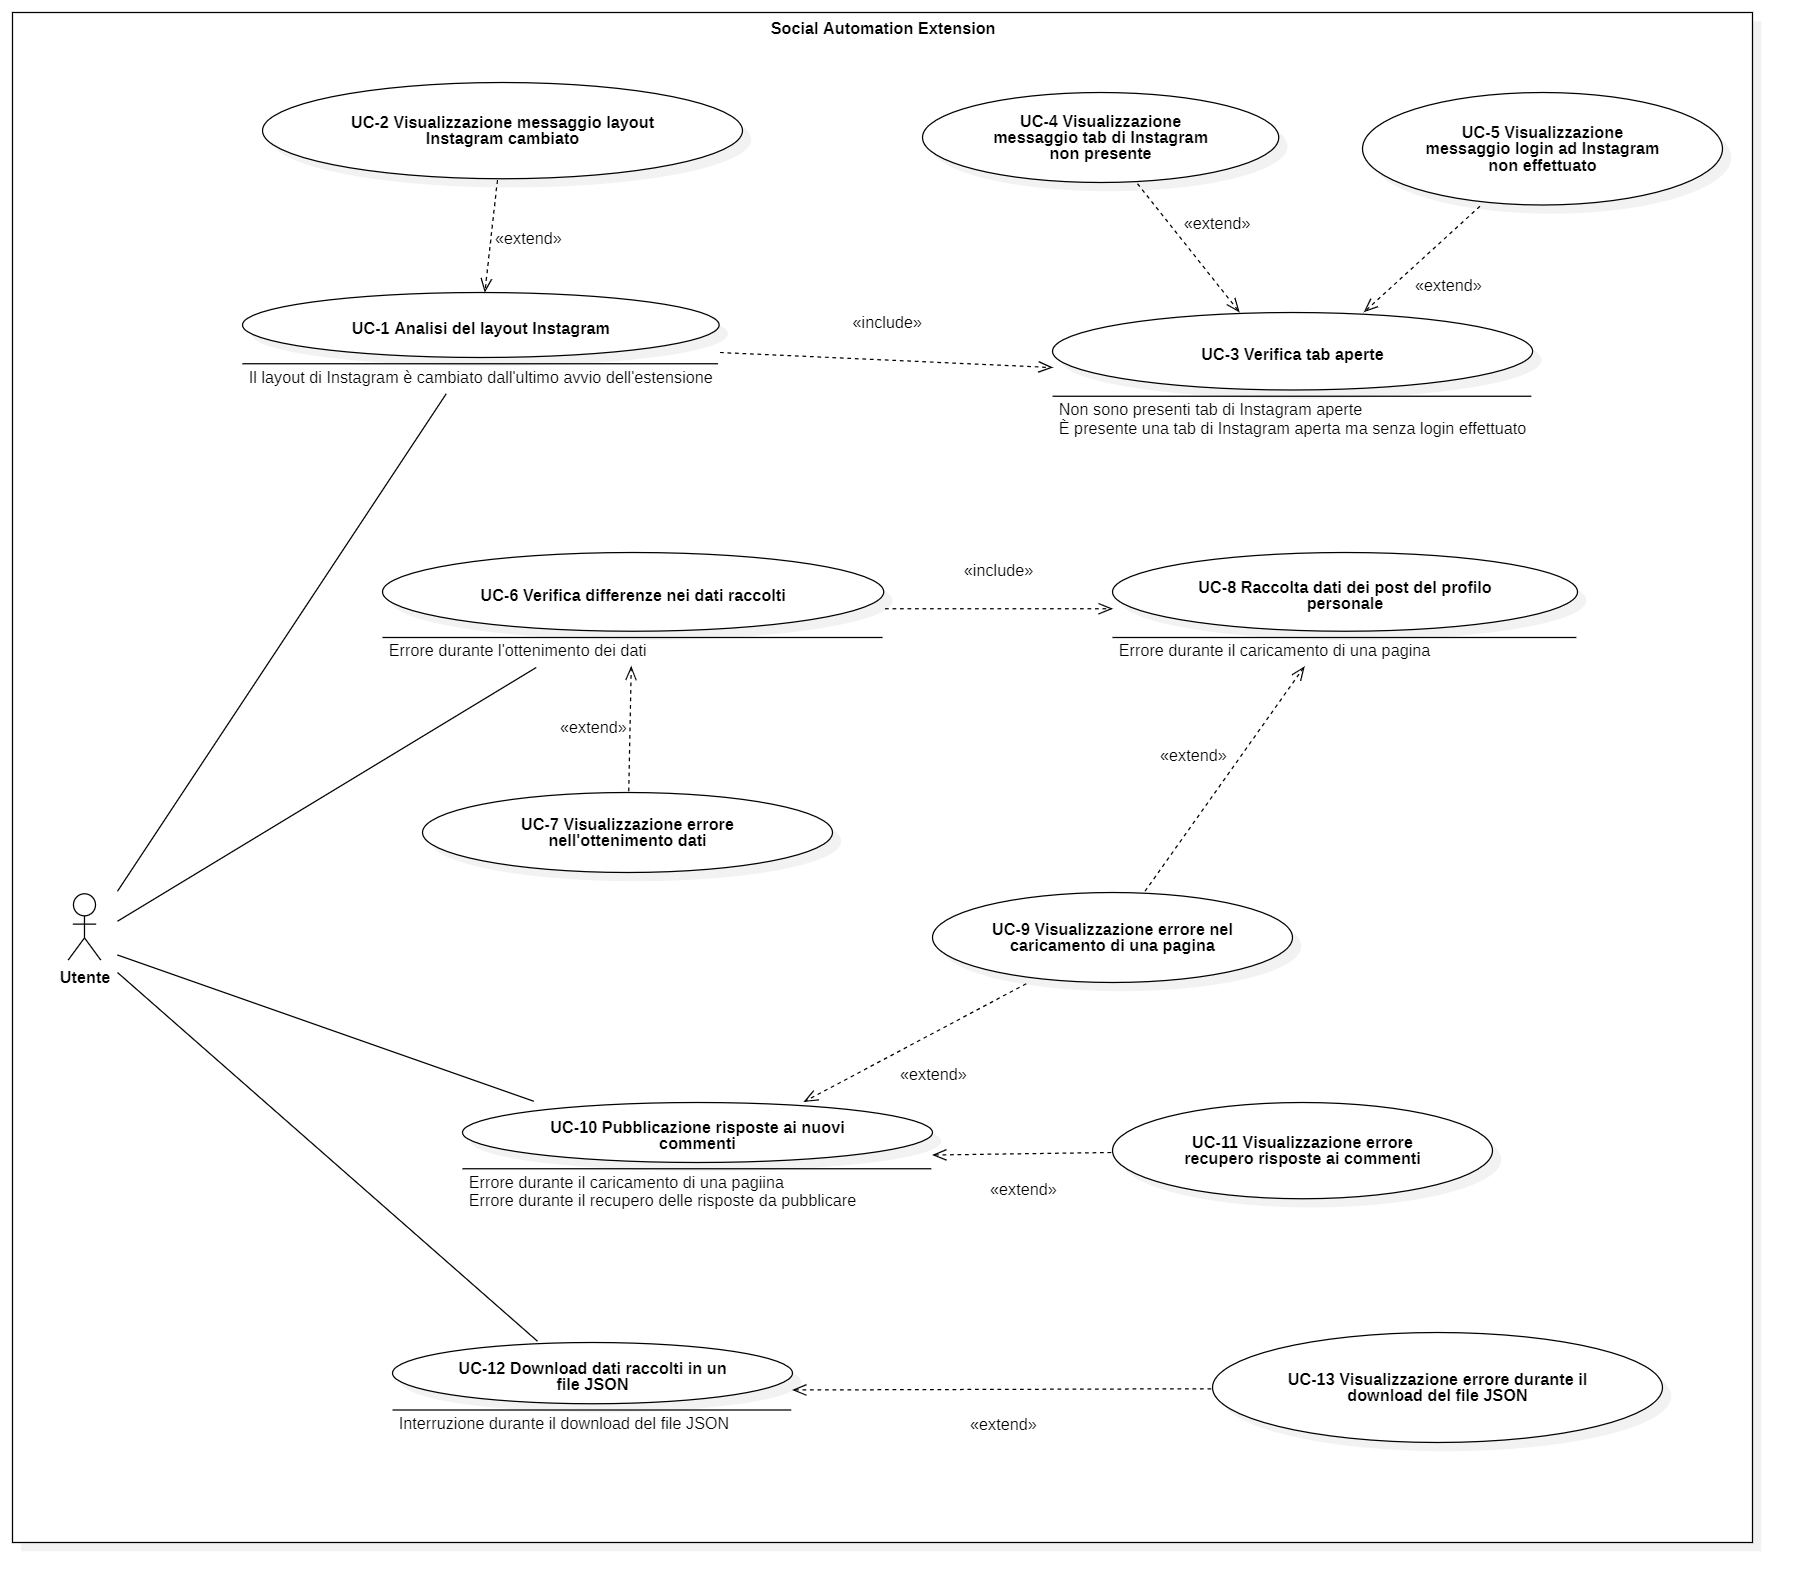
\includegraphics[width=\linewidth]{Sezioni/UseCase/Immagini/Generale.png}
    \caption{Diagramma generale use case}
\end{figure}

\begin{usecase}{UC-1}{Analisi del layout Instagram} 
    \label{uc:UC-1}

    \pre{} 
    
    \post{
        \item Viene visualizzato il pulsante che permette la raccolta dei dati
    }

    \actor{Utente} 

    \trigger{L'utente ha premuto sull'icona dell'estensione Chrome} 

    \inc{\hyperref[uc:UC-3]{UC-3}}

    \base{} 

    \scenario{ 
        \item L'utente preme l'icona per avviare l'estensione Chrome
                    
        \item Il sistema verifica la presenza di una tab Instagram aperta con login effettuato seguendo \hyperref[uc:UC-3]{UC-3}
             
        \item Il sistema esegue l'analisi del layout della pagina di Instagram per rilevare modifiche dovute ad aggiornamenti della piattaforma web

        \item L'utente visualizza il pulsante per effettuare la raccolta dei dati del proprio profilo
    } 

    \subscenario{ 
        \item[3.1] Layout di Instagram variato rispetto l'ultimo utilizzo dell'estensione:
        \begin{itemize}
            \item \hyperref[uc:UC-2]{UC-2}
        \end{itemize}
    } 
  \end{usecase}
  
  \begin{usecase}{UC-2}{Visualizzazione messaggio layout Instagram cambiato} 
    \label{uc:UC-2}

    \pre{
        \item Il sistema ha rilevato modifiche al layout di Instagram dovute a un aggiornamento della piattaforma web
    } 
    
    \post{
        \item Viene visualizzato un messaggio di errore che indica la variazione del layout di Instagram rispetto all'ultimo utilizzo dell'estensione
        \item Non è permessa la raccolta dei dati del proprio profilo
    }

    \actor{Utente} 

    \trigger{Almeno un elemento previsto nel layout di Instagram non è stato trovato} 

    \inc{}

    \base{} 

    \scenario{
        \item Il sistema mostra un messaggio che indica la variazione del layout di Instagram
    } 

    \subscenario{} 
  \end{usecase}

  \begin{usecase}{UC-3}{Verifica tab aperte} 
    \label{uc:UC-3}

    \pre{
        \item Il sistema non ha informazioni riguardo le tab aperte
    } 
    
    \post{
        \item Il sistema ha determinato la presenza di almeno una tab di Instagram aperta e con login effettuato
    }

    \actor{Utente} 

    \trigger{Il sistema deve verificare la presenza di una tab di Instagram con login effettuato per iniziare l'analisi del layout} 

    \inc{}

    \base{} 

    \scenario{
        \item Il sistema verifica la presenza di almeno una tab di Instagram aperta
        \item Il sistema verifica che l'utente abbia già effettuato il login nel proprio profilo
    } 

    \subscenario{
        \item[1.1] Tab di Instagram non presente
        \begin{itemize}
            \item \hyperref[uc:UC-4]{UC-4}
        \end{itemize}
        \item[2.1] Login nel proprio profilo Instagram non effettuato
        \begin{itemize}
            \item \hyperref[uc:UC-5]{UC-5}
        \end{itemize}
    } 
  \end{usecase}

  \begin{usecase}{UC-4}{Visualizzazione messaggio tab di Instagram non presente} 
    \label{uc:UC-4}

    \pre{
        \item Il sistema ha iniziato la verifica delle tab aperte
    } 
    
    \post{
        \item Il sistema ha determinato l'assenza di una tab di Instagram aperta
        \item L'utente è a conoscenza dei requisiti per utilizzare le funzionalità dell'estensione
    }

    \actor{Utente} 

    \trigger{Il sistema non ha trovato tab di Instagram aperte} 

    \inc{}

    \base{} 

    \scenario{
        \item Il sistema mostra un messaggio che indica la necessità di aprire una tab di Instagram ed effettuare il login
    } 

    \subscenario{} 
  \end{usecase}

  \begin{usecase}{UC-5}{Visualizzazione messaggio login a Instagram non effettuato} 
    \label{uc:UC-5}

    \pre{
        \item Il sistema ha determinato la presenza di almeno una tab di Instagram aperta
    } 
    
    \post{
        \item Il sistema ha determinato che l'utente non ha effettuato il login al suo profilo Instagram
        \item L'utente è a conoscenza della necessità di effettuare il login per poter utilizzare le funzionalità dell'estensione
    }

    \actor{Utente} 

    \trigger{Il sistema ha rilevato una scheda di Instagram aperta, ma senza che sia effettuato l'accesso a un profilo} 

    \inc{}

    \base{} 

    \scenario{
        \item Il sistema mostra un messaggio che indica la necessità di effettuare il login al proprio profilo Instagram
    } 

    \subscenario{} 
  \end{usecase}

  \begin{usecase}{UC-6}{Verifica differenze nei dati raccolti} 
    \label{uc:UC-6}

    \pre{
        \item Il sistema ha traccia dei dati raccolti nell'ultima esecuzione
        \item Il sistema termina la nuova raccolta dati con successo
    } 
    
    \post{
        \item Il sistema verifica se, nell'ultima raccolta, sono stati acquisiti nuovi dati e informa l'utente
    }

    \actor{Utente} 

    \trigger{L'utente ha avviato l'analisi dei dati del proprio profilo} 

    \inc{\hyperref[uc:UC-8]{UC-8}}

    \base{} 

    \scenario{
        \item L'utente richiede di analizzare i dati del proprio profilo
        \item Il sistema tiene traccia degli ultimi dati raccolti
        \item Il sistema effettua la raccolta dei nuovi dati seguendo \hyperref[uc:UC-8]{UC-8}
        \item Il sistema calcola le differenze tra i nuovi dati raccolti e i dati precedenti
        \item L'utente visualizza un messaggio che indica se sono presenti nuovi dati 
    } 

    \subscenario{
        \item[2.1] Errore interno durante l'ottenimento dei dati acquisiti nell'ultima raccolta
        \begin{itemize}
            \item \hyperref[uc:UC-7]{UC-7}
        \end{itemize}
        \item[4.1] Errore interno durante l'ottenimento dei dati acquisiti nella raccolta appena terminata
        \begin{itemize}
            \item \hyperref[uc:UC-7]{UC-7}
        \end{itemize}
    } 
  \end{usecase}

  \begin{usecase}{UC-7}{Visualizzazione errore nell'ottenimento dei dati} 
    \label{uc:UC-7}

    \pre{
        \item Avviene un errore interno al sistema durante l'ottenimento dei dati gestiti da esso
    } 
    
    \post{
        \item L'utente è a conoscenza dell'errore interno avvenuto
    }

    \actor{Utente} 

    \trigger{Il sistema riscontra un errore interno durante l'ottenimento dei dati} 

    \inc{}

    \base{} 

    \scenario{
        \item Il sistema notifica all'utente, mediante un messaggio di errore, la causa dell'anomalia
    } 

    \subscenario{} 
  \end{usecase}

  \begin{usecase}{UC-8}{Raccolta dati dei post del profilo personale} 
    \label{uc:UC-8}

    \pre{
        \item L'analisi del layout di Instagram è terminata con successo
    } 
    
    \post{
        \item Il sistema ha salvato i nuovi dati relativi ai post del profilo Instagram personale
    }

    \actor{Utente} 

    \trigger{L'utente ha premuto il pulsante per iniziare la raccolta dati} 

    \inc{}

    \base{} 

    \scenario{
        \item L'utente preme il pulsante per avviare una nuova raccolta dati
        \item Il sistema naviga il profilo dell'utente e raccoglie per ogni post: URL, numero, caption, src immagine, numero di like e lista dei commenti (autore e testo)
        \item Il sistema salva i dati raccolti
    } 

    \subscenario{
        \item[2.1] Tempo di caricamento eccessivo della pagina di un post
        \begin{itemize}
            \item \hyperref[uc:UC-9]{UC-9}
        \end{itemize}
    } 
  \end{usecase}

  \begin{usecase}{UC-9}{Visualizzazione errore nel caricamento di una pagina} 
  \label{uc:UC-9}

    \pre{
        \item Il caricamento di una pagina di un post durante la raccolta dati richiede un tempo eccessivo
    } 
    
    \post{
        \item L'utente è a conoscenza del problema riscontrato
    }

    \actor{Utente} 

    \trigger{Il tempo di caricamento della pagina di un post supera il timeout impostato} 

    \inc{}

    \base{} 

    \scenario{
        \item Viene mostrato un messaggio di errore che informa l'utente su quanto accaduto
    } 

    \subscenario{} 
  \end{usecase}

  \begin{usecase}{UC-10}{Pubblicazione risposte ai nuovi commenti} 
  \label{uc:UC-10}

    \pre{
        \item Il sistema ha terminato una raccolta dati e confrontando i risultati con la raccolta precedente ha rilevato differenze
    } 
    
    \post{
        \item Vengono pubblicate le risposte automatiche ai nuovi commenti rilevati
    }

    \actor{Utente} 

    \trigger{L'utente ha richiesto di pubblicare le risposte ai nuovi commenti rilevati} 

    \inc{}

    \base{} 

    \scenario{
        \item L'utente preme il pulsante per pubblicare le risposte automatiche
        \item Il sistema recupera una risposta da associare per ogni nuovo commento rilevato
        \item Il sistema ricerca ogni commento all'interno dei post e pubblica la risposta
        \item L'utente visualizza un messaggio di conferma della pubblicazione delle risposte
    } 

    \subscenario{
        \item[3.1] Errore durante il recupero delle risposte da pubblicare ai commenti
        \begin{itemize}
            \item \hyperref[uc:UC-11]{UC-11}
        \end{itemize}
        \item[3.1] Tempo di caricamento eccessivo della pagina di un post
        \begin{itemize}
            \item \hyperref[uc:UC-9]{UC-9}
        \end{itemize}
    } 
  \end{usecase}

  \begin{usecase}{UC-11}{Visualizzazione errore recupero risposte ai commenti} 
  \label{uc:UC-11}

    \pre{
        \item Avviene un errore interno al sistema durante il recupero delle risposte da pubblicare ai commenti
    } 
    
    \post{
        \item L'utente è a conoscenza dell'errore interno avvenuto
    }

    \actor{Utente} 

    \trigger{Il sistema riscontra un errore interno durante l'ottenimento delle risposte da pubblicare} 

    \inc{}

    \base{} 

    \scenario{
        \item Il sistema notifica all'utente, mediante un messaggio di errore, la causa dell'anomalia
    } 

    \subscenario{} 
  \end{usecase}

  \begin{usecase}{UC-12}{Download dati raccolti in un file JSON} 
  \label{uc:UC-12}

    \pre{
        \item Il sistema ha terminato una raccolta dati e confrontando i risultati con la raccolta precedente ha rilevato differenze
    } 
    
    \post{
        \item Viene scaricato un file JSON contenente i nuovi dati raccolti
    }

    \actor{Utente} 

    \trigger{L'utente ha richiesto il download del file JSON con i nuovi dati raccolti} 

    \inc{}

    \base{} 

    \scenario{
        \item L'utente preme il pulsante per scaricare il file JSON
        \item Il sistema avvia il download
        \item L'utente visualizza un messaggio di successo del download del file
    } 

    \subscenario{
        \item[2.1] Interruzione durante il download del file JSON richiesto
        \begin{itemize}
            \item \hyperref[uc:UC-13]{UC-13}
        \end{itemize}
    } 
  \end{usecase}

  \begin{usecase}{UC-13}{Visualizzazione errore durante il download del file JSON} 
  \label{uc:UC-13}

    \pre{
        \item Avviene un'interruzione durante il download del file JSON
    }

    \post{
        \item L'utente è a conoscenze dell'interruzione avvenuta
    }

    \actor{Utente} 

    \trigger{Il sistema rileva un'interruzione durante il download del file} 

    \inc{}

    \base{} 

    \scenario{
        \item Il sistema comunica all'utente, mediante un messaggio di errore, che si è verificata un'interruzione
    } 

    \subscenario{} 
  \end{usecase}

  



\section{Requisiti Software}
\label{sec:requisiti_software}
In questa sezione vengono elencati i requisiti software individuati per la realizzazione del progetto.
I requisiti sono stati definiti tramite l'analisi degli use case individuati e le riunioni con il tutor aziendale.
I requisiti software si dividono in:
\begin{enumerate}
    \label{en:req_type}
    \item Requisiti funzionali: definiscono le funzionalità attese dal sistema.
    \item Requisiti non funzionali: definiscono gli attributi attesi del sistema nel suo insieme.
    Si dividono in:
    \begin{enumerate}
        \item Requisiti di qualità: impongono dei vincoli sulla qualità del prodotto.
        \item Requisiti di vincolo: impongono dei vincoli sullo svolgimento del progetto.
    \end{enumerate}
\end{enumerate}
Ogni requisito software viene descritto indicando le seguenti informazioni:
\begin{enumerate}
    \item Identificativo che segue la sintassi:
    \begin{lstlisting}
        R<T><O/F>-<N>
    \end{lstlisting}
    Dove:
    \begin{enumerate}
        \item \lstinline{T} indica il tipo di requisito software che può variare tra \lstinline{F}(funzionali), \lstinline{Q}(di qualità) e \lstinline{V}(di vincolo).
        \item \lstinline{O} indica che il requisito è obbligatorio mentre \lstinline{F} indica che il requisito è facoltativo.
        \item \lstinline{N} è un numero crescente rispetto al tipo di requisito che parte dal valore 1.
    \end{enumerate}
    \item Descrizione testuale.
    \item Specifica, ovvero la lista di sotto requisiti che approfondiscono il requisito software principale.
    Ogni sotto requisito è identificato usando l'identificativo del requisito padre a cui viene aggiunto in coda un secondo numero crescente che parte da 1 (preceduto da un punto).
    \item Una lista degli use case che hanno dato origine al requisito software.
\end{enumerate}

\subsection{Requisiti funzionali}
\label{subsec:requisiti_funzionali}
I requisiti funzionali sono raggruppati usando una divisione ad alto livello del sistema in due componenti, ovvero 
\begin{enumerate}
    \item Logica di presentazione: si occupa della presentazione delle informazioni agli utenti.
    \item Logica di business: si occupa dell'elaborazione delle informazioni mostrate agli utenti e ottenute dagli utenti.
\end{enumerate}

\subsubsection{Logica di presentazione}

\paragraph{Obbligatori}

\begin{freq}
    {RFO-1}
    {Il sistema deve permettere la visualizzazione di un messaggio che indica lo stato delle tab aperte}
    \label{rf:RFO-1}%

    \subreq{RFO-1.1}{\hyperref[uc:UC-4]{UC-4}}{Il sistema deve visualizzare un messaggio che indica l'assenza di una tab di Instagram aperta}
    \subreq{RFO-1.2}{\hyperref[uc:UC-5]{UC-5}}{Il sistema deve visualizzare un messaggio che indica l'assenza del login nella tab di Instagram aperta}
\end{freq}

\begin{freq}
    {RFO-2}
    {Il sistema deve poter visualizzare gli elementi necessari per permettere la raccolta dei dati}
    \label{rf:RF2-3}%

    \subreq{RFO-2.1}{\hyperref[uc:UC-8]{UC-8}}{Il sistema deve visualizzare un pulsante che permetta di iniziare la raccolta dati}
\end{freq}

\begin{freq}
    {RFO-3}
    {Il sistema deve poter visualizzare gli elementi necessari per notificare l'esito della raccolta dati}
    \label{rf:RFO-3}%

    \subreq{RFO-3.1}{\hyperref[uc:UC-8]{UC-8}}{Il sistema deve visualizzare un messaggio che informa l'utente che la raccolta dei dati è in esecuzione}
    \subreq{RFO-3.2}{\hyperref[uc:UC-8]{UC-8}}{Il sistema deve visualizzare un messaggio che indica il successo della raccolta dati}
    \subreq{RFO-3.3}{\hyperref[uc:UC-8]{UC-8}}{Il sistema deve visualizzare un link all pagina dell'ultimo post di cui sono stati raccolti i dati}
    \subreq{RFO-3.4}{\hyperref[uc:UC-8]{UC-8}}{Il sistema deve visualizzare un messaggio che indica il numero di post di cui sono stati raccolti i dati e il numero di post totale del profilo}
    \subreq{RFO-3.5}{\hyperref[uc:UC-9]{UC-9}}{Se il caricamento della pagina di un post durante la raccolta non viene completato nei tempi previsti, il sistema deve visualizzare un messaggio che informa l'utente dell'errore}
\end{freq}

\begin{freq}
    {RFO-4}
    {Il sistema deve poter visualizzare gli elementi necessari per permettere la pubblicazione delle risposte ai nuovi commenti rilevati}
    \label{rf:RFO-4}%

    \subreq{RFO-4.1}{\hyperref[uc:UC-10]{UC-10}}{Il sistema deve visualizzare un pulsante che permetta di iniziare la pubblicazione delle risposte ai nuovi commenti}
\end{freq}

\begin{freq}
    {RFO-5}
    {Il sistema deve poter visualizzare gli elementi necessari per notificare l'esito della pubblicazione delle risposte ai nuovi commenti}
    \label{rf:RFO-5}%

    \subreq{RFO-5.1}{\hyperref[uc:UC-10]{UC-10}}{Il sistema deve visualizzare un messaggio che informa l'utente che la pubblicazione delle risposte è in esecuzione}
    \subreq{RFO-5.2}{\hyperref[uc:UC-10]{UC-10}}{Il sistema deve visualizzare un messaggio che indica il successo della pubblicazione delle risposte ai commenti}
    \subreq{RFO-5.3}{\hyperref[uc:UC-9]{UC-9}}{Se il caricamento della pagina di un post durante la pubblicazione non viene completato nei tempi previsti, il sistema deve visualizzare un messaggio che informa l'utente dell'errore}
    \subreq{RFO-5.4}{\hyperref[uc:UC-11]{UC-11}}{Se si verifica un errore durante il recupero delle risposte ai commenti da pubblicare, il sistema deve visualizzare un messaggio che informa l'utente dell'errore}
\end{freq}

\begin{freq}
    {RFO-6}
    {Il sistema deve poter visualizzare gli elementi necessari per permettere il download dei dati raccolti in un file JSON}
    \label{rf:RFO-6}%

    \subreq{RFO-6.1}{\hyperref[uc:UC-12]{UC-12}}{Il sistema deve visualizzare un pulsante che permetta di iniziare il download del file JSON con i nuovi dati raccolti}
    \subreq{RFO-6.2}{\hyperref[uc:UC-12]{UC-12}}{Il sistema deve visualizzare una finestra di dialogo che permetta di selezionare la cartella dove salvare il file}

\end{freq}

\begin{freq}
    {RFO-7}
    {Il sistema deve visualizzare gli elementi necessari per notificare l'esito del download del file}
    \label{rf:RFO-7}%

    \subreq{RFO-7.1}{\hyperref[uc:UC-12]{UC-12}}{Il sistema deve visualizzare un messaggio che indica il successo del download del file JSON}
    \subreq{RFO-7.2}{\hyperref[uc:UC-13]{UC-13}}{Se il download del file viene interrotto, il sistema deve visualizzare un messaggio che informa l'utente dell'interruzione}
\end{freq}

\paragraph{Facoltativi}

\begin{freq}
    {RFF-1}
    {Il sistema deve permettere la visualizzazione di un messaggio che indica il risultato dell'analisi del layout di Instagram}
    \label{rf:RFF-1}%

    \subreq{RFF-1.1}{\hyperref[uc:UC-1]{UC-1}}{Il sistema deve visualizzare un messaggio che informa l'utente che l'analisi del layout di Instagram è in esecuzione}
    \subreq{RFF-1.2}{\hyperref[uc:UC-1]{UC-1}}{Se l'analisi del layout di Instagram ha esito positivo, il sistema deve mostrare un messaggio che ne conferma il successo}
    \subreq{RFF-1.3}{\hyperref[uc:UC-2]{UC-2}}{Se l'analisi del layout di Instagram ha esito negativo, il sistema deve visualizzare un messaggio che indica l'impossibilità di effettuare una raccolta dati}
    \subreq{RFO-1.4}{\hyperref[uc:UC-2]{UC-2}}{Se l'analisi del layout di Instagram ha esito negativo, il sistema deve visualizzare un messaggio che indica ogni elemento del layout Instagram non trovato}
\end{freq}

\begin{freq}
    {RFF-2}
    {Il sistema deve poter visualizzare gli elementi necessari per notificare l'esito del calcolo delle differenze tra i dati raccolti}
    \label{rf:RFF-2}%

    \subreq{RFO-2.1}{\hyperref[uc:UC-6]{UC-6}}{Se vengono rilevate differenze tra i dati dell'ultima raccolta e quelli della raccolta precedente, il sistema deve visualizzare un messaggio che informa l'utente della presenza di variazioni nei nuovi dati raccolti}
    \subreq{RFO-2.2}{\hyperref[uc:UC-6]{UC-6}}{Se non vengono rilevate differenze tra i dati dell'ultima raccolta e quelli della raccolta precedente, il sistema deve visualizzare un messaggio che informa l'utente che i nuovi dati raccolti coincidono con quelli precedenti}
    \subreq{RFO-2.3}{\hyperref[uc:UC-7]{UC-7}}{Se si verifica un errore durante l'ottenimento dei dati delle ultime due raccolte, il sistema deve visualizzare un messaggio che informa l'utente dell'errore}
\end{freq}

\subsubsection{Logica di business}

\paragraph{Obbligatori}

\begin{freq}
    {RFO-8}
    {Il sistema deve poter gestire la persistenza dei dati raccolti}
    \label{rf:RFO-8}%

    \subreq{RFO-8.1}{\hyperref[uc:UC-8]{UC-8}}{Il sistema deve poter salvare in modo persistente i dati ottenuti durante una raccolta}
    \subreq{RFO-8.2}{\hyperref[uc:UC-6]{UC-6}, \hyperref[uc:UC-8]{UC-8}, \hyperref[uc:UC-12]{UC-12}}{Il sistema deve poter ottenere i dati salvati durante l'ultima raccolta}
\end{freq}

\begin{freq}
    {RFO-9}
    {Il sistema deve poter gestire le tab aperte}
    \label{rf:RFO-9}%

    \subreq{RFO-9.1}{\hyperref[uc:UC-3]{UC-3}}{Il sistema deve poter ottenere una lista delle tab aperte nella finestra del Browser}
    \subreq{RFO-9.2}{\hyperref[uc:UC-4]{UC-4}}{Il sistema deve poter ottenere l'URL di ogni tab aperta}
    \subreq{RFO-9.3}{\hyperref[uc:UC-4]{UC-4}}{Il sistema deve poter verificare se l'URL di una tab aperta corrisponde a un dominio di Instagram}
    \subreq{RFO-9.4}{\hyperref[uc:UC-5]{UC-5}}{Il sistema deve essere in grado di acquisire i cookie da una tab aperta}
    \subreq{RFO-9.5}{\hyperref[uc:UC-5]{UC-5}}{Il sistema deve controllare che siano presenti i cookie di autenticazione di Instagram}
\end{freq}

\begin{freq}
    {RFO-10}
    {Il sistema deve poter navigare tra le pagine di Instagram}
    \label{rf:RFO-10}%

    \subreq{RFO-10.1}{\hyperref[uc:UC-8]{UC-8}, \hyperref[uc:UC-10]{UC-10}}{Il sistema deve poter ottenere il pulsante nel layout Instagram per accedere alla pagina del profilo personale}
    \subreq{RFO-10.2}{\hyperref[uc:UC-8]{UC-8}}{Il sistema deve poter ottenere il numero di post totali pubblicati nel profilo personale}
    \subreq{RFO-10.3}{\hyperref[uc:UC-8]{UC-8}, \hyperref[uc:UC-10]{UC-10}}{Il sistema deve poter ottenere il link per caricare l'ultimo post pubblicato nel profilo personale}
    \subreq{RFO-10.4}{\hyperref[uc:UC-8]{UC-8}, \hyperref[uc:UC-10]{UC-10}}{Il sistema deve poter ottenere il pulsante nel layout Instagram per navigare al post successivo}
    \subreq{RFO-10.5}{\hyperref[uc:UC-8]{UC-8}, \hyperref[uc:UC-10]{UC-10}, \hyperref[uc:UC-9]{UC-9}}{Il sistema deve poter determinare il cambiamento dell'URL della pagina}
    \subreq{RFO-10.6}{\hyperref[uc:UC-8]{UC-8}, \hyperref[uc:UC-10]{UC-10}}{Il sistema deve poter determinare cambiamenti avvenuti al DOM della pagina}
\end{freq}

\begin{freq}
    {RFO-11}
    {Il sistema deve poter ottenere i dati di un post di Instagram}
    \label{rf:RFO-11}%

    \subreq{RFO-11.1}{\hyperref[uc:UC-8]{UC-8}}{Il sistema deve poter ottenere il numero del post}
    \subreq{RFO-11.2}{\hyperref[uc:UC-8]{UC-8}}{Il sistema deve poter ottenere la caption del post}
    \subreq{RFO-11.3}{\hyperref[uc:UC-8]{UC-8}}{Il sistema deve poter ottenere il numero di likes al post}
    \subreq{RFO-11.4}{\hyperref[uc:UC-8]{UC-8}, \hyperref[uc:UC-10]{UC-10}}{Il sistema deve poter ottenere l'URL della pagina del post}
    \subreq{RFO-11.5}{\hyperref[uc:UC-8]{UC-8}}{Il sistema deve poter ottenere il valore dell'attributo "src" nel caso in cui il post sia un'immagine}
    \subreq{RFO-11.6}{\hyperref[uc:UC-8]{UC-8}, \hyperref[uc:UC-10]{UC-10}}{Il sistema deve poter ottenere testo e autore di tutti i commenti al post che non contengono solo immagini}
    \subreq{RFO-11.7}{\hyperref[uc:UC-8]{UC-8}, \hyperref[uc:UC-10]{UC-10}}{Il sistema deve poter ottenere il pulsante per caricare i nuovi commenti}

\end{freq}

\begin{freq}
    {RFO-12}
    {Il sistema deve poter pubblicare una risposta ad un commento su un post di Instagram}
    \label{rf:RFO-12}%

    \subreq{RFO-12.1}{\hyperref[uc:UC-10]{UC-10}}{Il sistema deve poter identificare il commento corrispondente dato il testo, l'autore e l'URL del post in cui è pubblicato}
    \subreq{RFO-12.2}{\hyperref[uc:UC-10]{UC-10}}{Il sistema deve poter ottenere il pulsante per rispondere ad un commento}
    \subreq{RFO-12.3}{\hyperref[uc:UC-10]{UC-10}}{Il sistema deve poter ottenere l'area di testo in cui inserire il testo della risposta}
    \subreq{RFO-12.4}{\hyperref[uc:UC-10]{UC-10}}{Il sistema deve poter inserire correttamente il testo della risposta nell'area di testo}
    \subreq{RFO-12.5}{\hyperref[uc:UC-10]{UC-10}}{Il sistema deve poter ottenere il pulsante per pubblicare la risposta al commento}
    \subreq{RFO-12.6}{\hyperref[uc:UC-10]{UC-10}, \hyperref[uc:UC-11]{UC-11}}{Il sistema deve poter ottenere le risposte ai commenti da pubblicare}

\end{freq}

\begin{freq}
    {RFO-13}
    {Il sistema deve poter gestire il download di un file JSON}
    \label{rf:RFO-13}%

    \subreq{RFO-13.1}{\hyperref[uc:UC-12]{UC-12}}{Il sistema deve poter effettuare il download di un file nel file system locale}
    \subreq{RFO-13.2}{\hyperref[uc:UC-13]{UC-13}}{Il sistema deve poter determinare lo stato del download in corso}
\end{freq}

\paragraph{Facoltativi}

\begin{freq}
    {RFF-3}
    {Il sistema deve poter analizzare il layout di Instagram}
    \label{rf:RFF-3}%

    \subreq{RFF-3.1}{\hyperref[uc:UC-1]{UC-1}}{Il sistema deve poter aprire una tab di Instagram temporanea di un account di test}
    \subreq{RFF-3.2}{\hyperref[uc:UC-1]{UC-1}, \hyperref[uc:UC-2]{UC-2}}{Il sistema deve essere in grado di verificare che ciascun selettore di un elemento della pagina di Instagram individui correttamente l'elemento corrispondente nella pagina dell'account di test}
\end{freq}

\begin{freq}
    {RFF-4}
    {Il sistema deve gestire le differenze tra i dati raccolti nelle esecuzioni consecutive}
    \label{rf:RFF-4}%

    \subreq{RFF-4.1}{\hyperref[uc:UC-6]{UC-6}}{Il sistema deve poter calcolare le differenze tra due set di dati raccolti}
    \subreq{RFF-4.2}{\hyperref[uc:UC-6]{UC-6}}{Il sistema deve rappresentare le differenze calcolate in un formato JSON strutturato}
\end{freq}

\subsection{Requisiti non funzionali}
\label{subsec:requisiti_non_funzionali}

\subsubsection{Requisiti di vincolo}

\paragraph{Obbligatori}
\label{rnf:RVO-1}%
\nfreq{RVO-1}{Il sistema deve essere prodotto come estensione Chrome}{Discussione con tutor aziendale}
\label{rnf:RVO-2}%
\nfreq{RVO-2}{Il sistema deve essere supportato dall'ultima major version del browser Chrome}{Discussione con tutor aziendale}
\label{rnf:RVO-3}%
\nfreq{RVO-3}{Il progetto deve essere reso disponibile tramite GitHub}{Discussione con tutor aziendale}

\newpage
\subsubsection{Requisiti di qualità}

\paragraph{Obbligatori}

\label{rnf:RQO-1}%
\nfreq{RQO-1}{L'utente deve poter aprire e chiudere l'estensione in modo rapido e intuitivo}{Discussione con tutor aziendale}
\label{rnf:RQO-2}%
\nfreq{RQO-2}{I selettori utilizzati per il parsing della pagina web devono essere indipendenti dalla lingua e ben isolati nel codice}{Discussione con tutor aziendale}

\paragraph{Facoltativi}
\label{rnf:RQF-1}%
\nfreq{RQF-1}{L'estensione deve rimanere attiva su tutte le tab}{Discussione con tutor aziendale}
\label{rnf:RQF-2}%
\nfreq{RQF-2}{L'estensione deve rimanere attiva e garantire il suo corretto funzionamento anche quando l'utente interagisce con altre schede o pagine all'interno della stessa finestra del browser}{Discussione con tutor aziendale}


   



\end{document}